\section{Pervasive Computing}
Currently, computing is \textbf{computer-centric}. This requires users to:
\begin{itemize}
	\item Learn new technologies and interfaces
	\item Perform configuration and customisation
	\item Manage devices and applications	
\end{itemize}
No consensus on name:
\begin{itemize}
	\item Pervasive Computing
	\item Ubiquitous Computing
	\item Invisible Computing (rarely used)	
\end{itemize}

\begin{figure}[h]
	\centering
	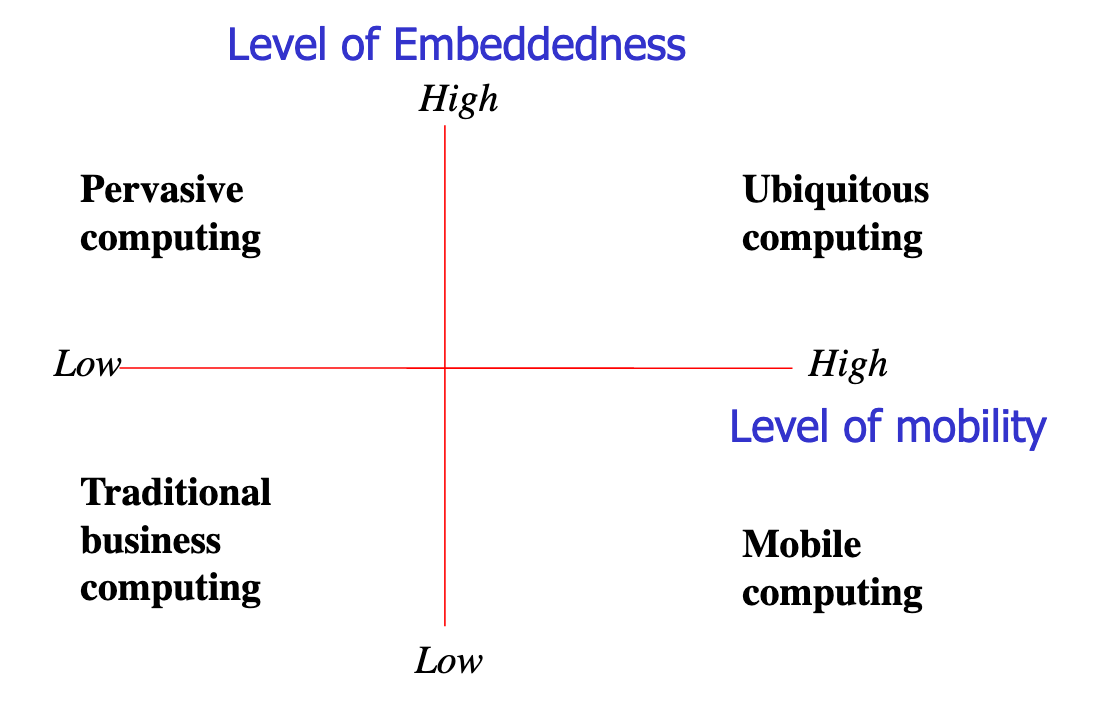
\includegraphics[width=0.8\linewidth]{definitions}
	\caption{Example Definition (not widely accepted)}
\end{figure}

\subsection{Pervasive Computing Paradigm}
\begin{itemize}
	\item Vision of future computing proposed in late 1980's
	\item Everyday objects (e.g. lamps, coffee cups, soup cans, ...) get computing ability
	\item Ideally, all these objects are wirelessly connected
	\item \textbf{User-centric approach to computing:} focus on users and their requirements
	\item The ultimate goal: computing when and where you need it provided through a network of unobtrusive devices
\end{itemize}
\vspace{2em}
\begin{itemize}
	\item Pervasive Computing offers \textbf{seamless computing} via:
	\begin{itemize}
		\item Self-configuration
		\item Awareness of circumstances (context) surrounding tasks
		\item Self-adaptation if context changes
	\end{itemize}
	\item The 6As model of pervasive computing: ``The \textbf{a}uthorized access to \textbf{a}nytime-\textbf{a}nywhere-\textbf{a}ny device-\textbf{a}ny network-\textbf{a}ny data''	
\end{itemize}

\subsubsection{Requirements}
Seamless computing supporting
\begin{itemize}
	\item mobility (users, devices, applications)
	\item network and device independence
	\item provision of QoS (wide range of QoS types)
	\item compensation for system ``failures''
	\item accommodation of changing user requirements and preferences
	\item security, privacy	
\end{itemize}
Intelligent support for user tasks:
\begin{itemize}
	\item context aware-applications
	\item awareness supported by
	\begin{itemize}
		\item system's knowledge about networks and devices
		\item context data from sensors
		\item user defined/inferred context
		\begin{itemize}
			\item QoS requirements of applications
			\item user preferences
			\item user activities
		\end{itemize}
	\end{itemize}	
\end{itemize}

\subsection{Context Definitions}
Context defined variously as:
\begin{itemize}
	\item An application/user's environment or situation
	\item A combination of computing, user and physical features	
\end{itemize}
Definition from Dey \& Abowd:
\begin{leftbar}
	``Context is any information that can be used to characterise the situation of an entity. An entity is a person, place or object that is considered relevant to the interaction between a user and an application, including the user and the application themselves.''
\end{leftbar}
From the UQ/NICTA Pervasive Computing Group:
\begin{itemize}
	\item The \textbf{context} of a task is the set of circumstances surrounding it that are potentially of relevance to its completion
	\item A \textbf{context model} identifies a concrete subset of the context that is realistically attainable from sensors and users, and able to be exploited in the execution of the task
	\item \textbf{Context information} is a set of data, gathered from sensors, application and users, that conforms to a context model and provides a snapshot that approximates the real-world context at a given point in time	
\end{itemize}

\subsubsection{Relevant Services}
\begin{itemize}
	\item Presentation of information and services to the user (e.g. tourist/museum guide)
	\item Automatic execution of a service for a user (e.g. sensor triggered emergency help)
	\item Tagging of context to information to support later retrieval (e.g. reminder and note-taking)
	\item Intelligent houses
	\item Sensor based human activity recognition
	\subitem e.g. to monitor performance (sport, piano playing)
	\subitem support for independent living of elderly	
\end{itemize}

\subsection{Context Modelling}
\begin{itemize}
	\item So far, context-aware applications are built mostly on context information sensed from physical sensors
	\item Models for gathering sensed context information are reasonably well developed
	\item Many context-aware applications require combined sensed and non-sensed context
	\item General context models are required
	\subitem recently there has been a lot of research on activity recognition	
\end{itemize}

\subsubsection{Management}
\begin{itemize}
	\item Processing sensed context information is only part of the problem
	\item General context models are needed	
	\begin{itemize}
		\item to capture various types of context information
		\item to capture characteristics of context information
	\end{itemize}
	\item Context management techniques
	\begin{itemize}
		\item to serve large numbers of applications
		\item to reuse context information
	\end{itemize}
\end{itemize}

\subsection{Context Model}
\subsubsection{Sensed context}
\begin{itemize}
	\item low persistence
	\item may be inaccurate, unknown, or stale
	\item source of errors
	\begin{itemize}
		\item sensor failures
		\item network disconnections
		\item delays (in communication or processing)
	\end{itemize}	
\end{itemize}

\subsubsection{Static context}
\begin{itemize}
	\item valid long term
	\item no quality problems	
\end{itemize}

\subsubsection{Profiled context}
\begin{itemize}
	\item moderate persistence
	\item prone to staleness
	\item source of errors
	\subitem user omitting updates	
\end{itemize}

\subsubsection{Derived context}
\begin{itemize}
	\item variable persistence
	\item subject to errors and inaccuracies
	\item source of errors
	\subitem imperfect inputs
	\subitem oversimplification in derivation mechanisms	
\end{itemize}
\vspace{2em}

Context information needs temporal characteristics
\begin{itemize}
	\item past state
	\item current state
	\item future state
	\item changes in state over time	
\end{itemize}
Context model needs to capture a variety of dependencies
\begin{itemize}
	\item physical laws (e.g. bandwidth-power dependency)
	\item ownership
	\subitem who owns devices
	\subitem which computers have a license to run particular software
	\item derivation rules
	\subitem for derived context	
\end{itemize}
Type classification (static, profiled, sensed, derived) can support context management tasks including:
\begin{itemize}
	\item update management
	\item resolution of inconsistency	
\end{itemize}

\subsection{Adaptations}
Adaptations can be applied at various layers:
\begin{itemize}
	\item Applications
	\subitem internal adaptation
	\subitem external adaptation
	\item Middleware (e.g. reflective middleware)
	\item Networks (vertical handovers, routing)
	\item Operating systems (resource management)	
\end{itemize}

\subsubsection{Network Adaptation}
\begin{itemize}
	\item Context-aware vertical handovers of data and real time streams between networks (Ethernet, WLAN, Bluetooth, 3/4/5G)
	\begin{itemize}
		\item Routing adaptation
		\item Resource management adaptations
	\end{itemize}	
\end{itemize}

\subsubsection{Adaptation triggering model}
\begin{itemize}
	\item events -- notifications about context changes
	\item context change evaluation may trigger adaptation
	\item rule based triggering model used
	\item rules specify which action should be taken for particular context changes	
\end{itemize}

\subsection{Interaction Semantics}
\begin{itemize}
	\item Most pervasive applications/systems use notifications as a communication paradigm
	\begin{itemize}
		\item to support a triggering model
		\item to provide scalability
		\item to allow easy reconfiguration
	\end{itemize}
	\item Notification systems with flexible registration for events is required
	\item Pervasive systems also need to support queries (i.e. RMI)	
\end{itemize}


















